\documentclass[8pt,ignorenonframetext,]{beamer}
\setbeamertemplate{caption}[numbered]
\setbeamertemplate{caption label separator}{: }
\setbeamercolor{caption name}{fg=normal text.fg}
\beamertemplatenavigationsymbolsempty
\usepackage{lmodern}
\usepackage{amssymb,amsmath}
\usepackage{ifxetex,ifluatex}
\usepackage{fixltx2e} % provides \textsubscript
\ifnum 0\ifxetex 1\fi\ifluatex 1\fi=0 % if pdftex
\usepackage[T1]{fontenc}
\usepackage[utf8]{inputenc}
\else % if luatex or xelatex
\ifxetex
\usepackage{mathspec}
\else
\usepackage{fontspec}
\fi
\defaultfontfeatures{Ligatures=TeX,Scale=MatchLowercase}
\fi
% use upquote if available, for straight quotes in verbatim environments
\IfFileExists{upquote.sty}{\usepackage{upquote}}{}
% use microtype if available
\IfFileExists{microtype.sty}{%
\usepackage{microtype}
\UseMicrotypeSet[protrusion]{basicmath} % disable protrusion for tt fonts
}{}
\newif\ifbibliography
\usepackage{color}
\usepackage{fancyvrb}
\newcommand{\VerbBar}{|}
\newcommand{\VERB}{\Verb[commandchars=\\\{\}]}
\DefineVerbatimEnvironment{Highlighting}{Verbatim}{commandchars=\\\{\}}
% Add ',fontsize=\small' for more characters per line
\usepackage{framed}
\definecolor{shadecolor}{RGB}{248,248,248}
\newenvironment{Shaded}{\begin{snugshade}}{\end{snugshade}}
\newcommand{\KeywordTok}[1]{\textcolor[rgb]{0.13,0.29,0.53}{\textbf{{#1}}}}
\newcommand{\DataTypeTok}[1]{\textcolor[rgb]{0.13,0.29,0.53}{{#1}}}
\newcommand{\DecValTok}[1]{\textcolor[rgb]{0.00,0.00,0.81}{{#1}}}
\newcommand{\BaseNTok}[1]{\textcolor[rgb]{0.00,0.00,0.81}{{#1}}}
\newcommand{\FloatTok}[1]{\textcolor[rgb]{0.00,0.00,0.81}{{#1}}}
\newcommand{\ConstantTok}[1]{\textcolor[rgb]{0.00,0.00,0.00}{{#1}}}
\newcommand{\CharTok}[1]{\textcolor[rgb]{0.31,0.60,0.02}{{#1}}}
\newcommand{\SpecialCharTok}[1]{\textcolor[rgb]{0.00,0.00,0.00}{{#1}}}
\newcommand{\StringTok}[1]{\textcolor[rgb]{0.31,0.60,0.02}{{#1}}}
\newcommand{\VerbatimStringTok}[1]{\textcolor[rgb]{0.31,0.60,0.02}{{#1}}}
\newcommand{\SpecialStringTok}[1]{\textcolor[rgb]{0.31,0.60,0.02}{{#1}}}
\newcommand{\ImportTok}[1]{{#1}}
\newcommand{\CommentTok}[1]{\textcolor[rgb]{0.56,0.35,0.01}{\textit{{#1}}}}
\newcommand{\DocumentationTok}[1]{\textcolor[rgb]{0.56,0.35,0.01}{\textbf{\textit{{#1}}}}}
\newcommand{\AnnotationTok}[1]{\textcolor[rgb]{0.56,0.35,0.01}{\textbf{\textit{{#1}}}}}
\newcommand{\CommentVarTok}[1]{\textcolor[rgb]{0.56,0.35,0.01}{\textbf{\textit{{#1}}}}}
\newcommand{\OtherTok}[1]{\textcolor[rgb]{0.56,0.35,0.01}{{#1}}}
\newcommand{\FunctionTok}[1]{\textcolor[rgb]{0.00,0.00,0.00}{{#1}}}
\newcommand{\VariableTok}[1]{\textcolor[rgb]{0.00,0.00,0.00}{{#1}}}
\newcommand{\ControlFlowTok}[1]{\textcolor[rgb]{0.13,0.29,0.53}{\textbf{{#1}}}}
\newcommand{\OperatorTok}[1]{\textcolor[rgb]{0.81,0.36,0.00}{\textbf{{#1}}}}
\newcommand{\BuiltInTok}[1]{{#1}}
\newcommand{\ExtensionTok}[1]{{#1}}
\newcommand{\PreprocessorTok}[1]{\textcolor[rgb]{0.56,0.35,0.01}{\textit{{#1}}}}
\newcommand{\AttributeTok}[1]{\textcolor[rgb]{0.77,0.63,0.00}{{#1}}}
\newcommand{\RegionMarkerTok}[1]{{#1}}
\newcommand{\InformationTok}[1]{\textcolor[rgb]{0.56,0.35,0.01}{\textbf{\textit{{#1}}}}}
\newcommand{\WarningTok}[1]{\textcolor[rgb]{0.56,0.35,0.01}{\textbf{\textit{{#1}}}}}
\newcommand{\AlertTok}[1]{\textcolor[rgb]{0.94,0.16,0.16}{{#1}}}
\newcommand{\ErrorTok}[1]{\textcolor[rgb]{0.64,0.00,0.00}{\textbf{{#1}}}}
\newcommand{\NormalTok}[1]{{#1}}
\usepackage{graphicx,grffile}
\makeatletter
\def\maxwidth{\ifdim\Gin@nat@width>\linewidth\linewidth\else\Gin@nat@width\fi}
\def\maxheight{\ifdim\Gin@nat@height>\textheight0.8\textheight\else\Gin@nat@height\fi}
\makeatother
% Scale images if necessary, so that they will not overflow the page
% margins by default, and it is still possible to overwrite the defaults
% using explicit options in \includegraphics[width, height, ...]{}
\setkeys{Gin}{width=\maxwidth,height=\maxheight,keepaspectratio}

% Prevent slide breaks in the middle of a paragraph:
\widowpenalties 1 10000
\raggedbottom

\AtBeginPart{
\let\insertpartnumber\relax
\let\partname\relax
\frame{\partpage}
}
\AtBeginSection{
\ifbibliography
\else
\let\insertsectionnumber\relax
\let\sectionname\relax
\frame{\sectionpage}
\fi
}
\AtBeginSubsection{
\let\insertsubsectionnumber\relax
\let\subsectionname\relax
\frame{\subsectionpage}
}

\setlength{\parindent}{0pt}
\setlength{\parskip}{6pt plus 2pt minus 1pt}
\setlength{\emergencystretch}{3em}  % prevent overfull lines
\providecommand{\tightlist}{%
\setlength{\itemsep}{0pt}\setlength{\parskip}{0pt}}
\setcounter{secnumdepth}{0}

\title{Happy R - Investigations Spatiales et Cartographiques}
\subtitle{Suite et Poursuite de la présentation de Jessica du 17/11/17}
\author{Eric \& Isabelle}
\date{23 mars 2018}

\begin{document}
\frame{\titlepage}

\section{CRS (Merci à Nicolas SABY, Unité InfoSol, Orléans, cf.~sa
présentation atelier
RESSTE)}\label{crs-merci-a-nicolas-saby-unite-infosol-orleans-cf.sa-presentation-atelier-resste}

\begin{frame}{Un mille à l'équateur vaut une minute}

\begin{center}
  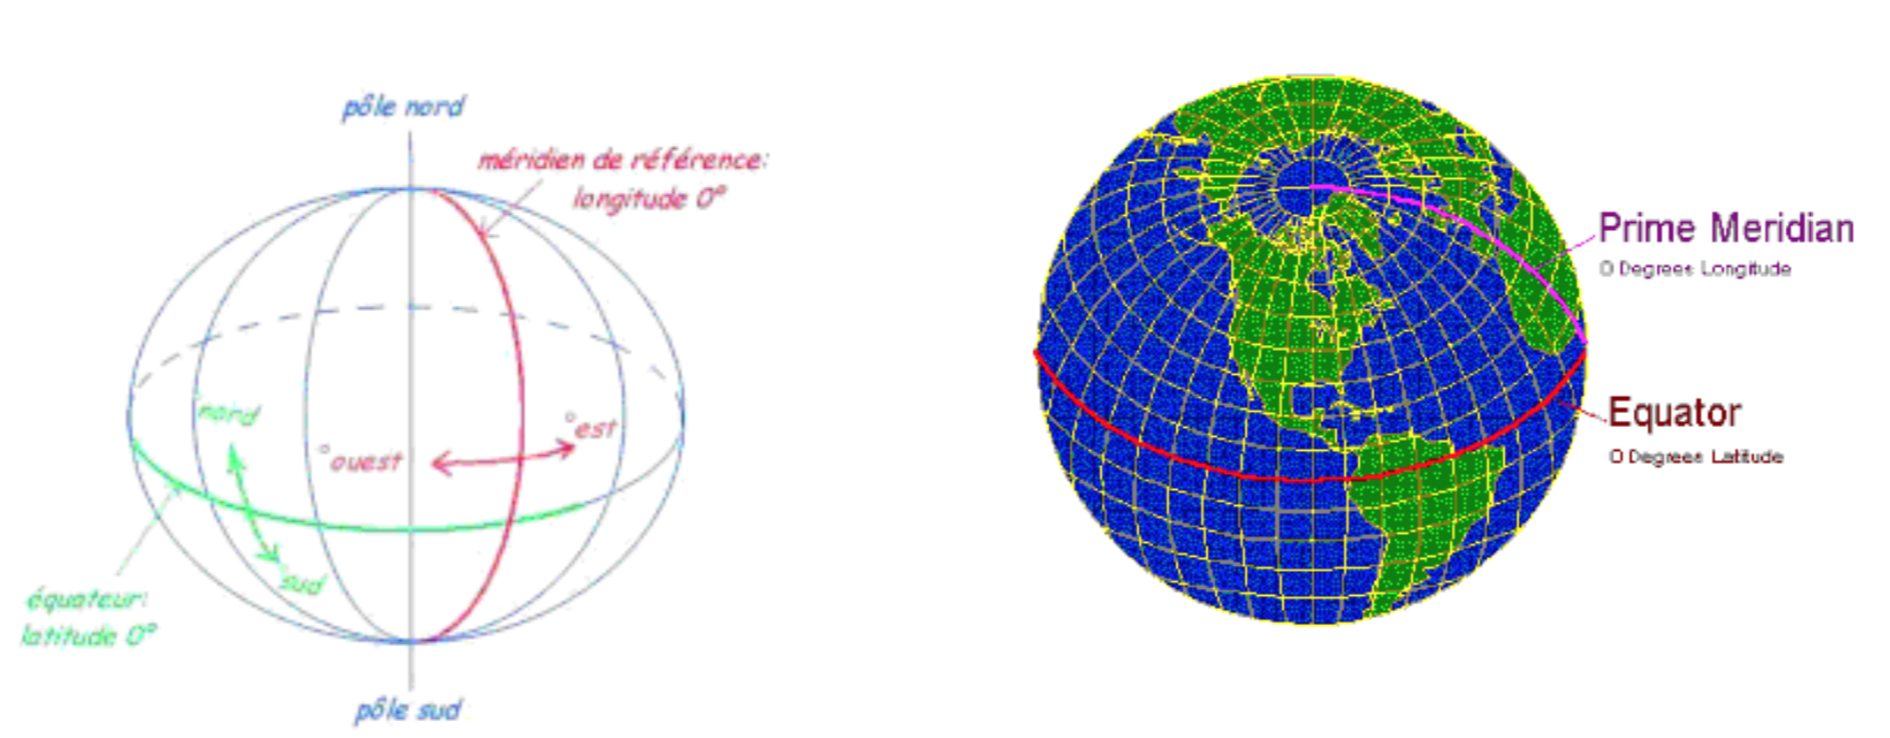
\includegraphics[height=0.45\textheight]{figSaby1_1.png} 
\end{center}\begin{center}
  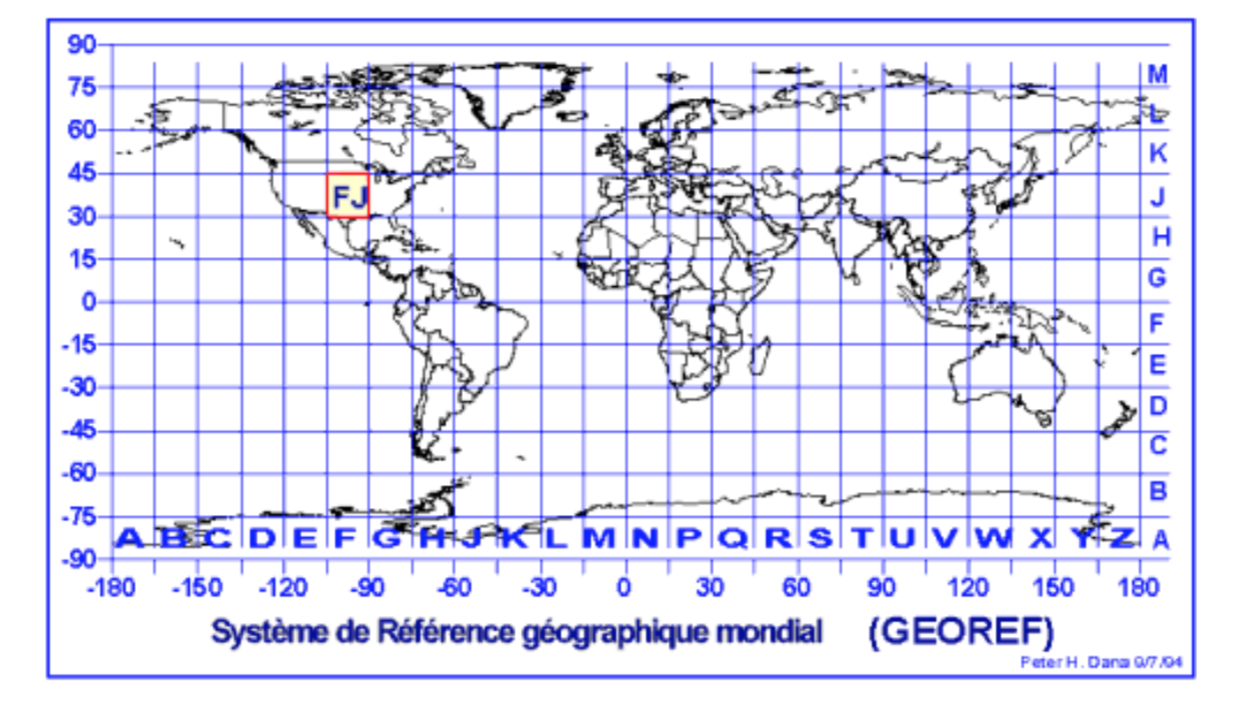
\includegraphics[height=0.4\textheight]{figSaby1_2.png}
\end{center}

\end{frame}

\begin{frame}{De multiples systèmes de projection}

\begin{center}
  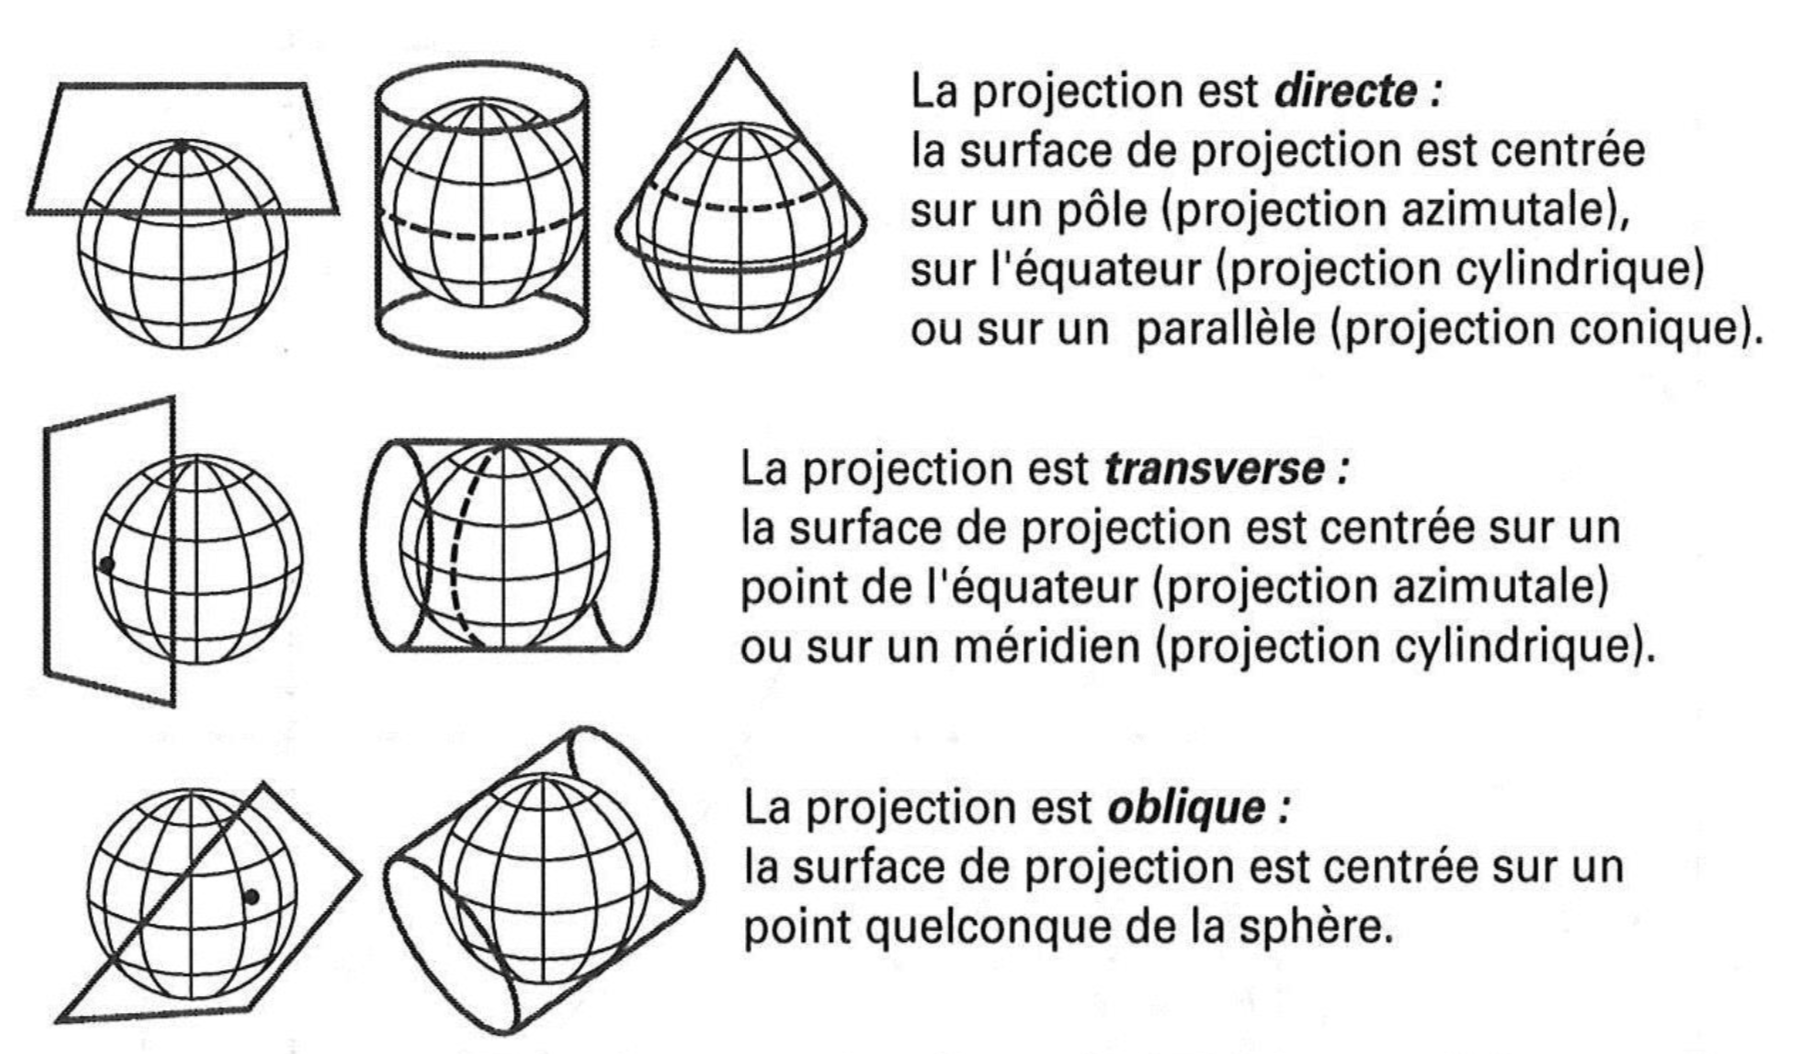
\includegraphics[width=0.9\textwidth]{figSaby2.png} 
\end{center}

\end{frame}

\begin{frame}{La France}

\begin{center}
  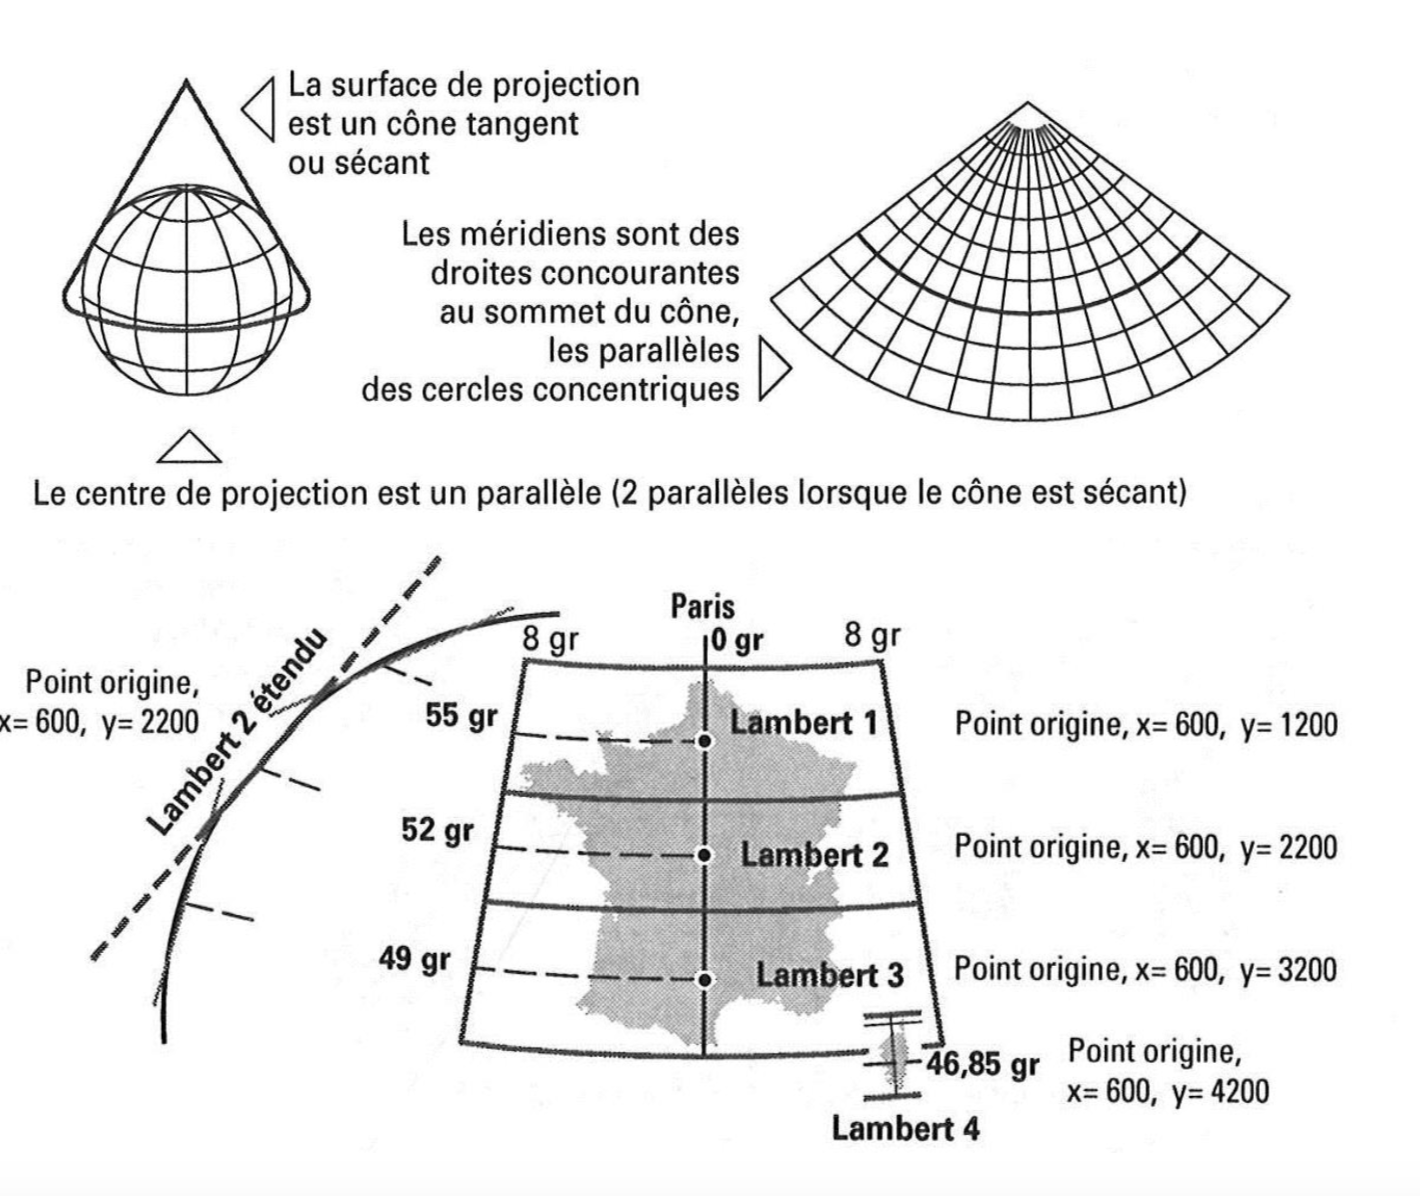
\includegraphics[width=0.9\textwidth]{figSaby3.png} 
\end{center}

\end{frame}

\begin{frame}[fragile]{En R , deux façons théoriques de définir le
système de projection}

\begin{itemize}
\item
  par le nom du code EPSG, par exemple WGS84 = 4326 (google) ou 2154
  (Lambert-93)
\item
  par l'écriture directe du code à considérer dans le slot proj4string
\end{itemize}

\begin{Shaded}
\begin{Highlighting}[]
\KeywordTok{CRSargs}\NormalTok{(}\KeywordTok{CRS}\NormalTok{(}\StringTok{"+init=epsg:2154"}\NormalTok{))}
\NormalTok{## [1] "+init=epsg:2154 +proj=lcc +lat_1=49 +lat_2=44 +lat_0=46.5 +lon_0=3 +x_0=700000 +y_0=6600000 +ellps=GRS80 +towgs84=0,0,0,0,0,0,0 +units=m +no_defs"}
\end{Highlighting}
\end{Shaded}

De fait, les objets spatiaux sont souvent dotés d'un CRS initial

\begin{Shaded}
\begin{Highlighting}[]
\KeywordTok{CRSargs}\NormalTok{(france@proj4string)}
\NormalTok{## [1] "+proj=longlat +ellps=WGS84"}
\end{Highlighting}
\end{Shaded}

Si on ne sait, on cherche dans gdal et/ou on va sur le net:
\url{http://spatialreference.org}

\begin{Shaded}
\begin{Highlighting}[]
\NormalTok{EPSG <-}\StringTok{ }\KeywordTok{make_EPSG}\NormalTok{()}
\NormalTok{EPSG_Lambert <-}\StringTok{ }\NormalTok{EPSG [}\KeywordTok{grep}\NormalTok{(}\StringTok{"Lambert"}\NormalTok{, EPSG$note), }\DecValTok{1}\NormalTok{:}\DecValTok{2}\NormalTok{] }
\KeywordTok{head}\NormalTok{(EPSG_Lambert)}
\NormalTok{##     code                                                        note}
\NormalTok{## 637 2138                             # NAD27(CGQ77) / Quebec Lambert}
\NormalTok{## 653 2154                                        # RGF93 / Lambert-93}
\NormalTok{## 654 2155 # American Samoa 1962 / American Samoa Lambert (deprecated)}
\NormalTok{## 684 2192                    # ED50 / France EuroLambert (deprecated)}
\NormalTok{## 686 2194 # American Samoa 1962 / American Samoa Lambert (deprecated)}
\NormalTok{## 809 2318                               # Ain el Abd / Aramco Lambert}
\end{Highlighting}
\end{Shaded}

\end{frame}

\begin{frame}[fragile]{En R , en pratique il faut \textbf{transformer}
les coordonnées via le système de projection}

\begin{itemize}
\tightlist
\item
  C'est le rôle de la fonction de reprojection \textbf{spTransform()}
\end{itemize}

\begin{Shaded}
\begin{Highlighting}[]
\KeywordTok{bbox}\NormalTok{(france)}
\NormalTok{##         min       max}
\NormalTok{## x -4.790282  9.562218}
\NormalTok{## y 41.364927 51.091109}
\NormalTok{france_Lambert93 <-}\StringTok{ }\KeywordTok{spTransform}\NormalTok{(france, }\KeywordTok{CRS}\NormalTok{(}\StringTok{"+init=epsg:2154"}\NormalTok{))}
\KeywordTok{bbox}\NormalTok{(france_Lambert93)}
\NormalTok{##         min     max}
\NormalTok{## x  124535.3 1242296}
\NormalTok{## y 6049526.6 7110717}
\end{Highlighting}
\end{Shaded}

\begin{itemize}
\item
  Cette reprojection est importante pour les calculs de distances
  (Variogrammes!)
\item
  Exercice: Paris a pour latitude : 48.866667 et pour longitude :
  2.333333. Quelles sont ses coordonnées sur une carte Lambert93?
  Quelles sont ses coordonnées en degrés, minutes, secondes
  (cf.~dd2dms). Celles de Bordeaux sont 48.866667 et 2.333333. Quelle
  est la distance entre ces deux villes (cf.~spDistsN1 et gzAzimuth)
\item
  Exercice: La grille des prévisions CHIMERE est donnée en coordonnées
  long/lat. Transformer l'objet spatial construit à l'exercice 3 en
  Lambert93 et visaliser les deux cartes obtenues pour voir l'effet de
  la projection conique.
\end{itemize}

\end{frame}

\section{Visualisation}\label{visualisation}

\begin{frame}[fragile]{Graphe interactif avec locator}

\begin{Shaded}
\begin{Highlighting}[]
\KeywordTok{plot}\NormalTok{(meuse_sp)}
\NormalTok{region <-}\StringTok{ }\KeywordTok{locator}\NormalTok{(}\DataTypeTok{type=}\StringTok{"o"}\NormalTok{)}
\CommentTok{#finir avec Esc}

\NormalTok{n <-}\StringTok{ }\KeywordTok{length}\NormalTok{(region$x)}
\NormalTok{p <-}\StringTok{ }\KeywordTok{Polygon}\NormalTok{(}\KeywordTok{cbind}\NormalTok{(region$x,region$y)[}\KeywordTok{c}\NormalTok{(}\DecValTok{1}\NormalTok{:n,}\DecValTok{1}\NormalTok{),], }\DataTypeTok{hole=}\OtherTok{FALSE}\NormalTok{)}
\NormalTok{ps <-}\StringTok{ }\KeywordTok{Polygons}\NormalTok{(}\KeywordTok{list}\NormalTok{(p), }\DataTypeTok{ID =} \StringTok{"region"}\NormalTok{)}
\NormalTok{sps <-}\StringTok{ }\KeywordTok{SpatialPolygons}\NormalTok{(}\KeywordTok{list}\NormalTok{(ps))}
\KeywordTok{plot}\NormalTok{(meuse_sp[sps,], }\DataTypeTok{pch=}\DecValTok{16}\NormalTok{, }\DataTypeTok{cex=}\DecValTok{1}\NormalTok{, }\DataTypeTok{add=}\OtherTok{TRUE}\NormalTok{, }\DataTypeTok{col=}\StringTok{"red"}\NormalTok{)}
\CommentTok{# Voir ?over}
\KeywordTok{plot}\NormalTok{(meuse_sp[!}\KeywordTok{is.na}\NormalTok{(}\KeywordTok{over}\NormalTok{(meuse_sp,sps)),], }\DataTypeTok{pch=}\DecValTok{16}\NormalTok{, }\DataTypeTok{cex=}\DecValTok{1}\NormalTok{, }\DataTypeTok{add=}\OtherTok{TRUE}\NormalTok{, }\DataTypeTok{col=}\StringTok{"blue"}\NormalTok{)}
\CommentTok{#}
\NormalTok{pointschoisis<-}\KeywordTok{identify}\NormalTok{(}\KeywordTok{coordinates}\NormalTok{(meuse_sp))}
\KeywordTok{print}\NormalTok{(pointschoisis)}
\end{Highlighting}
\end{Shaded}

\end{frame}

\begin{frame}{Graph interactif avec locator}

\begin{center}
  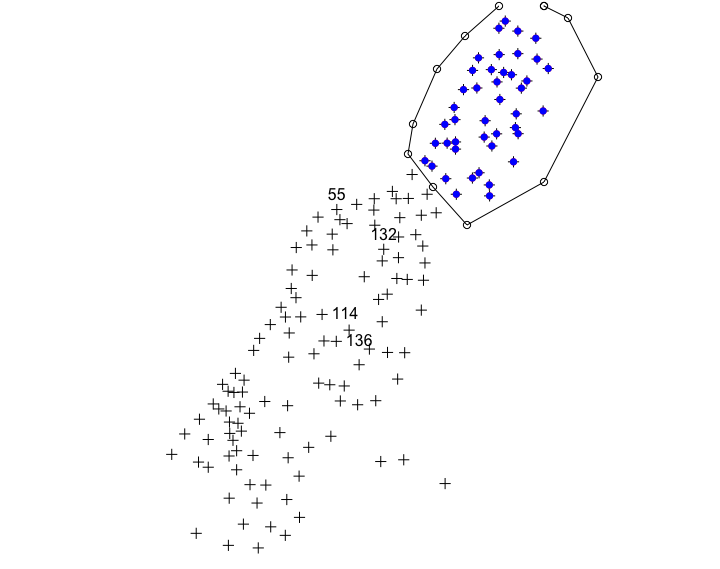
\includegraphics[width=0.9\textwidth]{figlocator.png} 
\end{center}

\end{frame}

\begin{frame}[fragile]{Visualisation treillis avec spplot}

\begin{Shaded}
\begin{Highlighting}[]
\KeywordTok{par}\NormalTok{(}\DataTypeTok{mfrow=}\KeywordTok{c}\NormalTok{(}\DecValTok{1}\NormalTok{,}\DecValTok{1}\NormalTok{))}
\KeywordTok{library}\NormalTok{(RColorBrewer)}
\NormalTok{bleus <-}\StringTok{ }\KeywordTok{brewer.pal}\NormalTok{(}\DecValTok{7}\NormalTok{, }\StringTok{"Blues"}\NormalTok{)}
\NormalTok{lead.st <-}\StringTok{ }\KeywordTok{as.vector}\NormalTok{(}\KeywordTok{scale}\NormalTok{(meuse$lead)); zinc.st <-}\StringTok{ }\KeywordTok{as.vector}\NormalTok{(}\KeywordTok{scale}\NormalTok{(meuse$zinc))}
\NormalTok{copper.st <-}\StringTok{ }\KeywordTok{as.vector}\NormalTok{(}\KeywordTok{scale}\NormalTok{(meuse$copper)); cadmium.st <-}\StringTok{ }\KeywordTok{as.vector}\NormalTok{(}\KeywordTok{scale}\NormalTok{(meuse$cadmium))}
\NormalTok{meuse.st<-}\KeywordTok{data.frame}\NormalTok{(}\DataTypeTok{x=}\NormalTok{meuse$x, }\DataTypeTok{y=}\NormalTok{meuse$y,lead.st,zinc.st,copper.st,cadmium.st)}
\KeywordTok{coordinates}\NormalTok{(meuse.st) <-}\StringTok{ }\ErrorTok{~}\NormalTok{x+y}
\NormalTok{cuts=}\KeywordTok{c}\NormalTok{(-}\FloatTok{1.2}\NormalTok{,}\DecValTok{0}\NormalTok{,}\DecValTok{1}\NormalTok{,}\DecValTok{2}\NormalTok{,}\DecValTok{3}\NormalTok{,}\DecValTok{5}\NormalTok{)}
\KeywordTok{spplot}\NormalTok{(meuse.st, }\KeywordTok{c}\NormalTok{(}\StringTok{"cadmium.st"}\NormalTok{, }\StringTok{"copper.st"}\NormalTok{, }\StringTok{"lead.st"}\NormalTok{, }\StringTok{"zinc.st"}\NormalTok{), }
             \DataTypeTok{key.space=}\StringTok{"right"}\NormalTok{, }\DataTypeTok{main =} \StringTok{"Standardised metallic deposits"}\NormalTok{, }\DataTypeTok{cex =} \NormalTok{.}\DecValTok{75}\NormalTok{,}
             \DataTypeTok{cuts =} \NormalTok{cuts, }\DataTypeTok{col.regions=}\NormalTok{bleus)}
\end{Highlighting}
\end{Shaded}

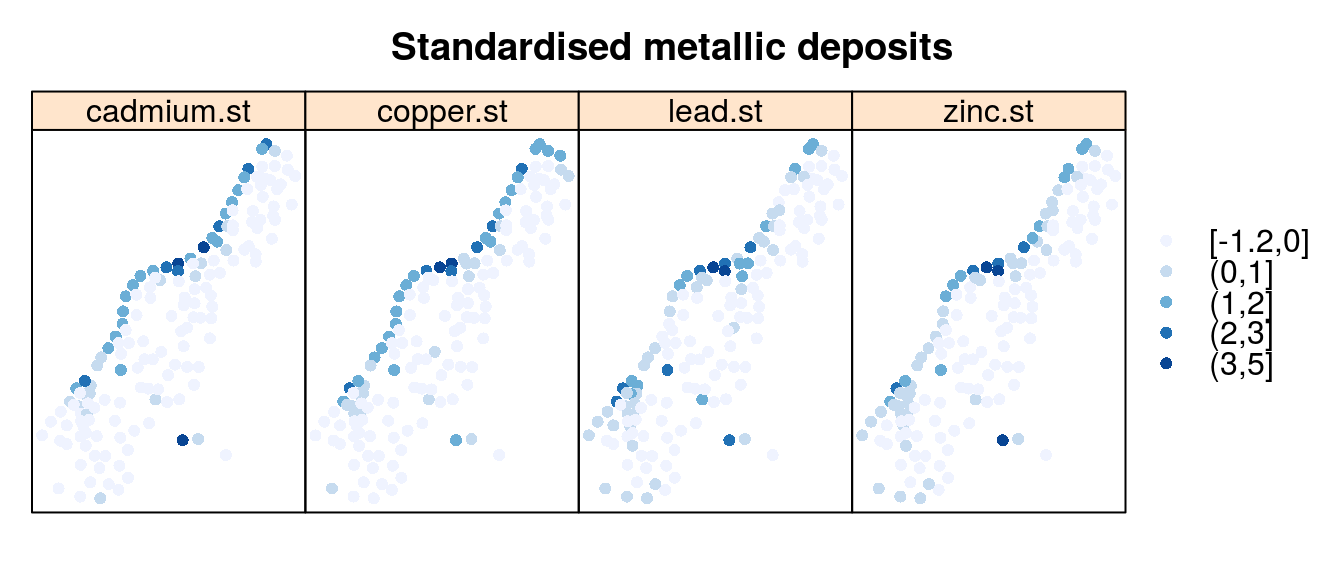
\includegraphics{happyR-230318-PLUS_files/figure-beamer/visuspplot1-1.pdf}

\end{frame}

\begin{frame}[fragile]{Visualisation spplot Kriege vs IDW}

\begin{Shaded}
\begin{Highlighting}[]
\KeywordTok{library}\NormalTok{(gstat)}
\NormalTok{zn <-}\StringTok{ }\KeywordTok{krige}\NormalTok{(zinc~}\DecValTok{1}\NormalTok{,meuse_sp,meuse_sg)}
\NormalTok{## [inverse distance weighted interpolation]}
\NormalTok{meuse_sg$zincIDW <-}\StringTok{ }\NormalTok{zn$var1.pred}

\NormalTok{vgmMeuse <-}\StringTok{ }\KeywordTok{variogram}\NormalTok{(zinc~}\DecValTok{1}\NormalTok{, meuse_sp, }\DataTypeTok{cutoff=}\DecValTok{1000}\NormalTok{)}
\NormalTok{vgmExpMeuse <-}\StringTok{ }\KeywordTok{fit.variogram}\NormalTok{(vgmMeuse, }\KeywordTok{vgm}\NormalTok{(}\DecValTok{150000}\NormalTok{, }\StringTok{"Exp"}\NormalTok{, }\DecValTok{1000}\NormalTok{, }\DecValTok{40000}\NormalTok{))}
\KeywordTok{plot}\NormalTok{(vgmMeuse, vgmExpMeuse, }\DataTypeTok{main=}\StringTok{"Exponential"}\NormalTok{, }\DataTypeTok{col=}\StringTok{'black'}\NormalTok{)}
\end{Highlighting}
\end{Shaded}

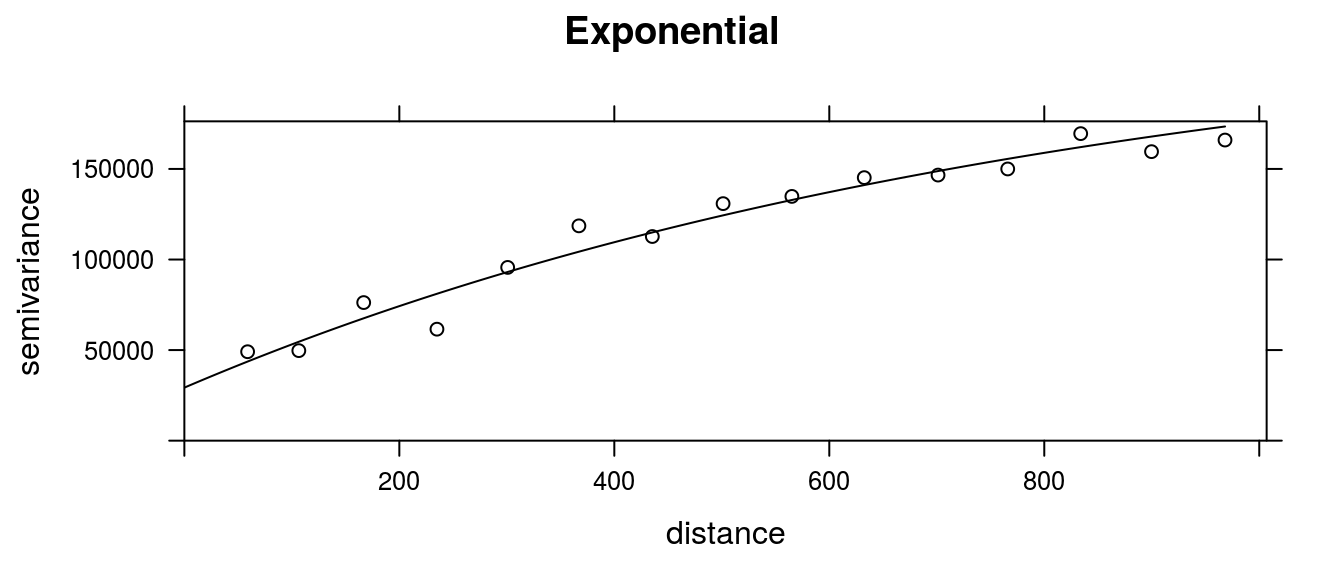
\includegraphics{happyR-230318-PLUS_files/figure-beamer/visuspplot2-1.pdf}

\begin{Shaded}
\begin{Highlighting}[]
\NormalTok{znkrige<-}\KeywordTok{krige}\NormalTok{(zinc~}\DecValTok{1}\NormalTok{, meuse_sp,meuse_sg, }\DataTypeTok{model=}\NormalTok{vgmExpMeuse)}
\NormalTok{## [using ordinary kriging]}
\NormalTok{meuse_sg$zincKRG <-}\StringTok{ }\NormalTok{znkrige$var1.pred}
\end{Highlighting}
\end{Shaded}

\end{frame}

\begin{frame}[fragile]{Construction de sp.layout}

\begin{Shaded}
\begin{Highlighting}[]
\NormalTok{river <-}\StringTok{ }\KeywordTok{list}\NormalTok{(}\StringTok{"sp.polygons"}\NormalTok{, meuse.riv_poly, }\DataTypeTok{col=}\StringTok{'darkblue'}\NormalTok{, }\DataTypeTok{fill=}\NormalTok{T)}
\NormalTok{north <-}\StringTok{ }\KeywordTok{list}\NormalTok{(}\StringTok{"SpatialPolygonsRescale"}\NormalTok{, }\KeywordTok{layout.north.arrow}\NormalTok{(), }\DataTypeTok{offset =} 
                \KeywordTok{c}\NormalTok{(}\DecValTok{178750}\NormalTok{,}\DecValTok{332500}\NormalTok{),}
              \DataTypeTok{scale =} \DecValTok{400}\NormalTok{)}
\NormalTok{scale <-}\StringTok{ }\KeywordTok{list}\NormalTok{(}\StringTok{"SpatialPolygonsRescale"}\NormalTok{, }\KeywordTok{layout.scale.bar}\NormalTok{(), }\DataTypeTok{offset =} 
                \KeywordTok{c}\NormalTok{(}\DecValTok{180200}\NormalTok{, }\DecValTok{329800}\NormalTok{), }\DataTypeTok{scale =} \DecValTok{1000}\NormalTok{, }\DataTypeTok{fill=}\KeywordTok{c}\NormalTok{(}\StringTok{"transparent"}\NormalTok{,}\StringTok{"black"}\NormalTok{))}
\NormalTok{txt1 <-}\StringTok{ }\KeywordTok{list}\NormalTok{(}\StringTok{"sp.text"}\NormalTok{, }\KeywordTok{c}\NormalTok{(}\DecValTok{180200}\NormalTok{, }\DecValTok{329950}\NormalTok{), }\StringTok{"0"}\NormalTok{)}
\NormalTok{txt2 <-}\StringTok{ }\KeywordTok{list}\NormalTok{(}\StringTok{"sp.text"}\NormalTok{, }\KeywordTok{c}\NormalTok{(}\DecValTok{181200}\NormalTok{, }\DecValTok{329950}\NormalTok{), }\StringTok{"1 km"}\NormalTok{)}
\NormalTok{pts <-}\StringTok{ }\KeywordTok{list}\NormalTok{(}\StringTok{"sp.points"}\NormalTok{, meuse_sp, }\DataTypeTok{pch =} \DecValTok{3}\NormalTok{, }\DataTypeTok{col =} \StringTok{"black"}\NormalTok{)}
\NormalTok{meuse.layout <-}\StringTok{ }\KeywordTok{list}\NormalTok{(river, north, scale, txt1, txt2, pts)}
\end{Highlighting}
\end{Shaded}

\end{frame}

\begin{frame}[fragile]{Visualisation sp.layout+spplot}

\begin{Shaded}
\begin{Highlighting}[]
\NormalTok{meuse.layout <-}\StringTok{ }\KeywordTok{list}\NormalTok{(river, north, scale, txt1, txt2, pts)}
\KeywordTok{spplot}\NormalTok{(meuse_sg, }\KeywordTok{c}\NormalTok{(}\StringTok{"zincIDW"}\NormalTok{, }\StringTok{"zincKRG"}\NormalTok{), }\DataTypeTok{sp.layout =} \NormalTok{meuse.layout, }\DataTypeTok{cuts=}\DecValTok{5}\NormalTok{, }\DataTypeTok{col.regions=}\NormalTok{bleus)}
\end{Highlighting}
\end{Shaded}

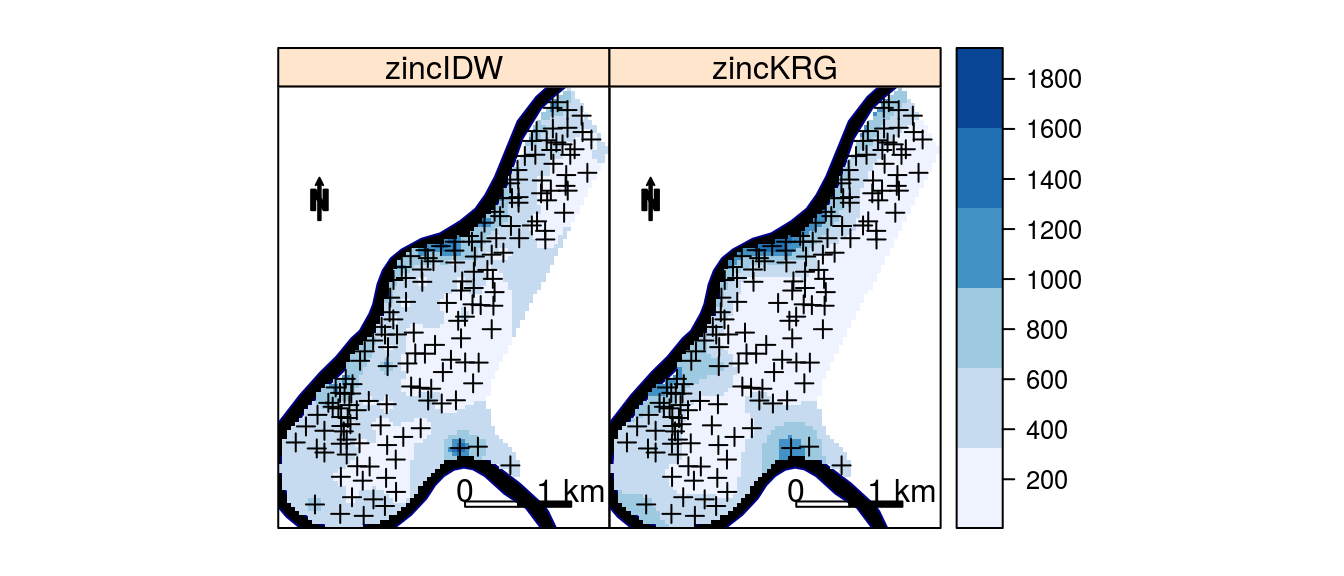
\includegraphics{happyR-230318-PLUS_files/figure-beamer/visuspplot4-1.pdf}

\end{frame}

\begin{frame}[fragile]{Pistes pour le futur}

\begin{enumerate}
\def\labelenumi{\arabic{enumi}.}
\item
  Explorer le \textbf{package \texttt{sf} } qui associe les
  fonctionalités de \texttt{sp}, \texttt{rgdal}, et \texttt{rgeos} en un
  seul package \emph{spatial features} fondé sur le principe
  \texttt{tidyverse}.
\item
  Les packages \textbf{outils}
  \texttt{rgeos},\texttt{rgdal},\texttt{maps},\texttt{maptools}\ldots{}
  Qui voudrait faire un tour d'horizon? La connection avec les outils
  SIG?
\item
  Continuer de comprendre la modélisation \textbf{geostatistique} et son
  inférence. L'étude des dépendances dans le modèle multinormal
  (d'observation ou latent) peut être approché sous l'angle de la:
\end{enumerate}

\begin{itemize}
\tightlist
\item
  \textbf{matrice de variance} qui analyse les corrélations spatiales
  sous forme de variogrammes (packages: structuré sur \texttt{sp}:
  \texttt{gstat}, ou indépendants:
  \texttt{spatial},\texttt{field},\texttt{RandomFields}, \texttt{GeoR},
  etc. )
\item
  \textbf{matrice de précision} qui décrit les indépendances
  conditionnelles (voir par exemple le package structuré sur
  \texttt{sp}: \texttt{spdep}) ou son utilisation pour les modèles
  géostatistiques complexes \texttt{INLA})
\end{itemize}

\begin{enumerate}
\def\labelenumi{\arabic{enumi}.}
\setcounter{enumi}{3}
\tightlist
\item
  \textbf{Extensions de la géostatistique } qui intéresseront le réseau
  RESSTE
\end{enumerate}

\begin{itemize}
\tightlist
\item
  \textbf{Le spatio-temporel} (packages: structuré sur \texttt{sp}:
  \texttt{spacetime}) sp+xts+data.frame=spacetime
\item
  \textbf{Approche Bayesiennes} (réplicats MCMC de structure de type
  cartes)
\end{itemize}

\end{frame}

\end{document}
